\chapter{成本}
\label{chp:cost}

\section{怎样看待和衡量成本}

\subsection{机会成本}

\begin{Definition}[机会成本]\index{cost 成本!opportunity cost 机会成本}
在面临多方案择一决策时,被舍弃的选项中的最高价值者是本次决策的机会成本。
\end{Definition}

草稿:opportunity cost opportunity lost,成本这个词语古已有之,至少在你学习经济学教科书之前就有了、就使用过。如果让你给经济活动的成本进行定义,你会不会把成本和花费联系起来,那么哪些花费该被划归经济学的范围。

草稿:生产函数吞进的要素的成本,而不是占有要素的成本。

以后提到的所有成本术语,潜台词都是从经济学的视角看待的成本,从机会成本的角度看待的成本。我们关注的是成本的来源——即要素,成本的数量——即次优的收益,而(暂时)不关注要素的所有者是谁,因为我们的研究目标是要素转变为产品的生产活动。

例如拍摄一部电影的成本是4000万人民币,这个数量对于穷人和富翁是不变的,即便你立刻可以从自己的账户支取4000万也不会使之拍摄电影这种生产活动的成本变为零。

为什么是4000万?因为拍摄电影的要素种类、价格是明确的——这里避免使用“确定的”以避免与“价格恒定”产生混淆。

为什么要素价格会明确为那个标准,或者说为什么要素会索要这个价格?因为他们为其他老板打工的最高价格就是这样,如果你不能满足他们,他们就会选择更优的渠道去实现自己的价格。一个更宽泛的假设是,即便他不从事影视行业他也会得到这个价格——虽然对于“人”这种要素来说很难重现。

机会成本又称为择一成本、替代性成本。机会成本对商业公司来说,可以是利用一定的时间或资源生产一种商品时,而失去的利用这些资源生产其他最佳替代品的机会就是机会成本。

在生活中,有些机会成本可用货币来衡量。例如,农民在获得更多土地时,如果选择养猪就不能选择养鸡,养猪的机会成本就是放弃养鸡的收益。但有些机会成本往往无法用货币衡量,例如,在图书馆看书学习还是享受电视剧带来的快乐之间进行选择。

而机会成本泛指一切在作出选择后其中一个最大的损失,机会成本会随付出的代价改变而作出改变,例如被舍弃掉的选项之喜爱程度或价值作出改变时,而得到之价值是不会令机会成本改变的。

而如果在选择中放弃选择最高价值的选项(首选),那么其机会成本将会是首选。而作出选择时,应该要选择最高价值的选项(机会成本最低的选项),而放弃选择机会成本最高的选项,即失去越少越明智。

\subsection{显成本与隐成本}
\index{cost 成本!explicit cost 显成本}
\index{cost 成本!implicit cost 隐成本}

机会成本通常包括两部分:
\begin{asparaenum}
\item 使用他人资源的机会成本,即付给资源拥有者的货币代价被称作显性成本。
\item 因为使用自有资源而放弃其他可能性中得到的最大回报的那个代价,也被称为隐性成本。
\end{asparaenum}

\subsection{经济成本与会计成本}
\index{cost 成本!economic cost 经济成本}
\index{cost 成本!accounting cost 会计成本}

机会成本与会计成本是两个不同的概念。

会计成本是指实际支付的货币成本。机会成本可能等于会计成本,也可能不等于会计成本。在完全竞争的条件下,机会成本等于会计成本;在商品(或生产要素)供应不足、实行配给的条件下,机会成本高于会计成本;在商品积压或要素闲置的条件下,机会成本低于会计成本,甚至为零。通常是在机会成本高于会计成本的情况下,使用机会成本的概念。
\begin{figure}[!h]
\colorbox{black!3}{\parbox{\linewidth-2\fboxsep}{%
\centering
\begin{tikzpicture}[x=0.75cm,y=0.333cm]
\fill[blue] (0,0) rectangle (11,3);			%会计成本
\fill[green!75] (11,0) rectangle (17,3);	%会计利润
\fill[blue] (0,3) rectangle (11,6);			%显成本
\fill[orange] (11,3) rectangle (14,6);		%隐成本
\fill[green] (14,3) rectangle (17,9);		%经济利润
\fill[red] (0,6) rectangle (14,9);			%经济成本
\draw[draw=blue!50] (0,3) -- (11,3);
\draw (5.5,1.5) node[white,font=\small\it] {会计成本};
\draw (14,1.5) node[white,font=\small\it] {会计利润};
\draw (5.5,4.5) node[white,font=\small\it] {显成本};
\draw (12.5,4.5) node[white,font=\small\it] {隐成本};
\draw (15.5,6) node[white,font=\small\it] {经济利润};
\draw (7,7.5) node[white,font=\small\it] {经济成本};
\end{tikzpicture}
\caption{机会成本角度的成本构成分析}
\label{fig:cost-structure-analysis-with-opportunity-cost}
}}
\end{figure}

\subsection{生产过程:长期与短期}
\index{cost 成本!variable cost 可变成本}
\index{cost 成本!fixed cost 不变成本}
\index{cost 成本!sunk cost 沉没成本}
\index{cost 成本!long run cost 长期成本}
\index{cost 成本!short run cost 短期成本}
在这里不能只理解到短期内不可变的成本成为固定成本,还要意识到后文的短期生产均衡中为什么用边际分析法讨论短期最优。

\section{短期成本}

\subsection[平均成本和边际成本]{平均成本和边际成本(三叉戟)}
\index{cost 成本!average cost 平均成本}
\index{cost 成本!marginal cost 边际成本}

\begin{figure}[!h]
\colorbox{black!3}{\parbox{\linewidth-2\fboxsep}{%
\centering
\begin{subfigure}[b]{0.5\textwidth}
\centering
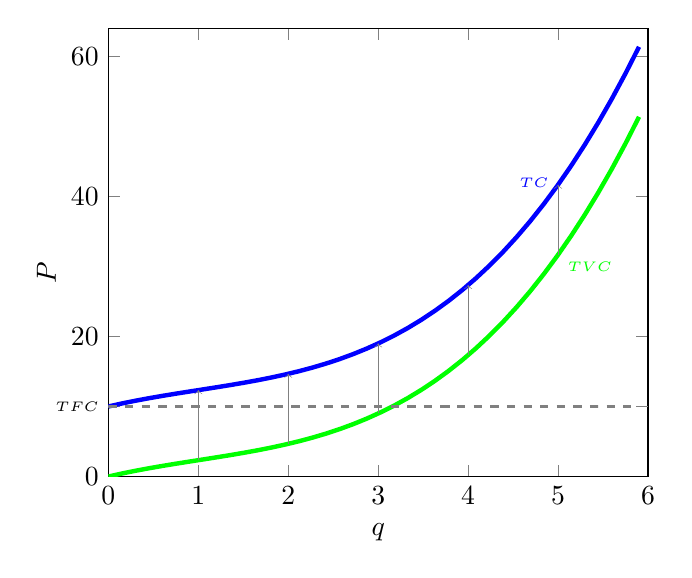
\begin{tikzpicture}
\begin{axis}[
	xmin=0,	xmax=6,	ymin=0,	ymax=64,
	extra y ticks={10},
	extra y tick labels={\tiny $TFC$},
	xlabel style={below},xlabel=$q$,ylabel style={left},ylabel=$P$,
	samples=40]
\addplot[green,ultra thick,domain=0:5.9] {(x^3)/3-x^2+3*x};
\addplot[blue,ultra thick,domain=0:5.9] {(x^3)/3-x^2+3*x+10};
\addplot[gray,thick,dashed,domain=0:5.9] {10};
\draw (axis cs:5,42) node[blue,left] {\tiny $TC$};
\draw (axis cs:5,32) node[green,below right] {\tiny $TVC$};
\addplot[->,gray,very thin] coordinates {(1,7/3) (1,37/3)};
\addplot[->,gray,very thin] coordinates {(2,14/3) (2,44/3)};
\addplot[->,gray,very thin] coordinates {(3,9) (3,19)};
\addplot[->,gray,very thin] coordinates {(4,52/3) (4,82/3)};
\addplot[->,gray,very thin] coordinates {(5,95/3) (5,125/3)};
\end{axis}
\end{tikzpicture}
    \caption{总成本}
	\label{fig:short-run-costs-curves-tctfctvc}%
\end{subfigure}%
\begin{subfigure}[b]{0.5\textwidth}
\centering
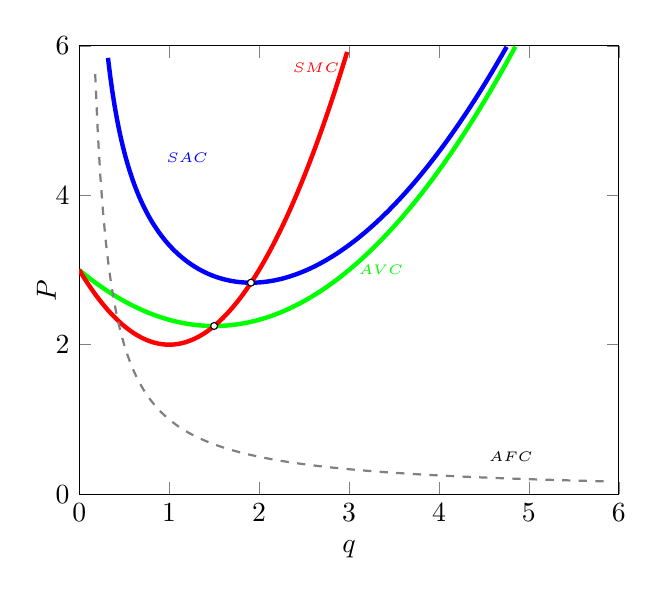
\begin{tikzpicture}
		\begin{axis}[
			xmin=0,xmax=6,ymin=0,ymax=6,restrict y to domain=0:6,
			xlabel style={below},xlabel=$q$,ylabel style={left},ylabel=$P$,
			samples=200]
			%AVC
			\addplot[ultra thick,domain=0:5,draw=green] {(x^2)/3-x+3};
				\draw (rel axis cs:0.5,0.5) node[green,right] {\tiny $AVC$};			%AVC
			\addplot[ultra thick,domain=0:4.9,draw=blue] {(x^2)/3-x+3+1/x};
				\draw (rel axis cs:0.2,0.75) node[blue] {\tiny $SAC$};				%SAC
			\addplot[ultra thick,domain=0:4.9,draw=red] {x^2-2*x+3};			%SMC
				\draw (rel axis cs:0.5,0.95) node[red,left] {\tiny $SMC$};
			\addplot[dashed,gray,thick,samples=200,domain=0:5.9] {1/x};				%AFC
				\draw (rel axis cs:0.8,0.05) node[above] {\tiny $AFC$};
			
			\addplot[only marks,forget plot,black,mark options={mark size=1.25pt,fill=white},mark=*] coordinates {
				(1.5,2.25)
				(1.91,2.83)
			};
		\end{axis}
	\end{tikzpicture}
    \caption{平均成本和边际成本}
	\label{fig:short-run-costs-curves-sacavcsmcafc}%
\end{subfigure}%
\caption{短期生产成本曲线}
\label{fig:short-run-costs-curves}%
	\caption*{将$TVC$曲线向上平移$TFC$个单位即可得到$TC$曲线。$SMC$、$SAC$、$AVC$可以是U型的,且$SMC$经过$SAC$、$AVC$的最低点。$AFC$总是递减的。}%
}}
\end{figure}

如图(\ref{fig:short-run-costs-curves})当$MC<AC$的时候, $A$C呈递减趋势;$MC>AC$的时候,$AC$呈递增趋势;$MC=AC$的时候,$AC$达到最低点,总有$MC$交$AC$于$AC$ 的最低点\footnote{%
注意:边际值与平均值交与后者的最低点只是特例,普遍关系是边际值对平均值的拉动关系,参见第\pageref{sec:average-and-marginal-function}页附录 \ref{sec:average-and-marginal-function}}。二者的关系可以表示为:
\begin{equation}
AC斜率=\frac{dAC}{dq} = \frac{MC-AC}{q}
\label{eq:average-and-marginal}
\end{equation}
也就是说$MC$曲线的变化要敏感于$AC$曲线的变化:不管上升或是下降,$MC$都要先于$AC$表现出来。在$MC$交于$AC$最低点后,$MC$会拉动$AC$ 一起上升;在交点之前,$MC$会拉$AC$一起下降。相关推导参看第\pageref{sec:average-and-marginal-function}页的附录。

\subsection{为什么短期供给曲线积分之后是总可变成本而非总成本}

短期总成本分为两部分,一是固定要素的总固定成本,而是可变要素的总可变成本,总成本的变化即边际成本完全是由可变要素带来的,故而边际成本加总之后只代表总可变成本。教学的话可以举小船排水量的例子:一只小船空船排水量为5,满载3人,每人排水量为1,则满载排水量(总排水)为$5+1+1+1=8$,边际排水量之和为$1+1+1=3$,固定排水量为$5$。

\begin{figure}[!h]
\colorbox{black!3}{\parbox{\linewidth-2\fboxsep}{%
\centering
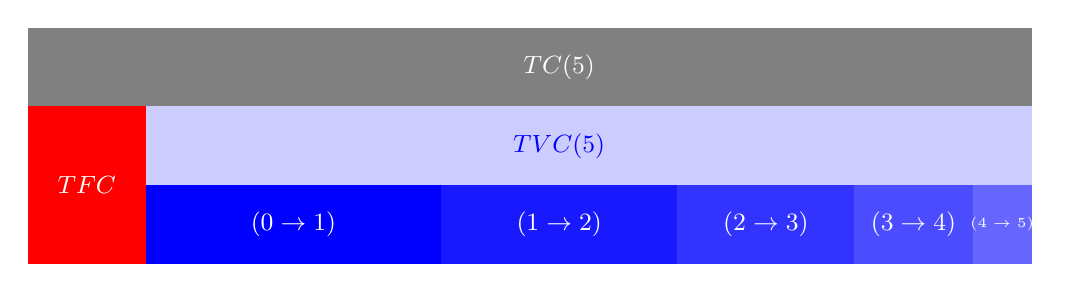
\begin{tikzpicture}[x=0.75cm,y=0.2cm]
\fill[red] (0,0) rectangle (-2,10);
\fill[blue] (0,0) rectangle (5,5);
\fill[blue!90] (5,0) rectangle (9,5);
\fill[blue!80] (9,0) rectangle (12,5);
\fill[blue!70] (12,0) rectangle (14,5);
\fill[blue!60] (14,0) rectangle (15,5);
\fill[blue!20] (0,5) rectangle (15,10);		%TVC
\fill[gray] (-2,10) rectangle (15,15);		%TC
\draw (7,12.5) node[white,font=\small] {$TC(5)$};
\draw (-1,5) node[white,font=\small] {$TFC$};
\draw (7,7.5) node[blue,font=\small] {$TVC(5)$};
\draw (2.5,2.50) node[white,font=\small] {$(0 \to 1)$};
\draw (7,2.50) node[white,font=\small] {$(1 \to 2)$};
\draw (10.5,2.50) node[white,font=\small] {$(2 \to 3)$};
\draw (13,2.50) node[white,font=\small] {$(3 \to 4)$};
\draw (14.5,2.50) node[white,font=\tiny] {$(4 \to 5)$};
\end{tikzpicture}
\caption{短期成本分析}
\label{fig:analysis-of-short-term-cost}
}}
\end{figure}

根据\emph{牛顿—莱布尼茨公式},假如$F(x)$是$f(x)$的一个原函数,
\[
\int_a^b f(x) = F(b) - F(a)\text{,}
\]
而$TC$和$TVC$都是$SMC$的原函数,
\[
TC(q)=TFC+TVC(q)
\]
其中$TFC$为常数($TFC=TC(0)$),则
\[
\frac{{dTC(q)}}{{dq}} = \frac{{dTVC(q)}}{{dq}} = SMC(q)
\]
故而,
\[
\int_0^{{q^ * }} SMC(q) = TC({q^*}) - TC(0) = TVC({q^*})\text{。}
\]


\section{长期成本}

\section*{推荐阅读}
\addcontentsline{toc}{section}{\hspace{-2.5em}推荐阅读}
\markright{推荐阅读}
\begin{asparaenum}
\item sallyax24. (2005-11-23). 边际成本与平均成本的关系. from \url{http://bbs.pinggu.org/thread-57129-1-1.html}
\item J皮尔庞特M. (2011-9-29). 边际成本下降时,平均成本为什么有可能上升. from \url{http://bbs.pinggu.org/thread-1192150-1-1.html}
\item 空城. (2012-4-17). 高手求教$MC$上升的时候$AC$曲线也上升么. from \url{http://bbs.pinggu.org/thread-1418817-1-1.html}
\end{asparaenum}

\newpage
\section*{本章附录}
\markright{本章附录}

\subsection*{连续函数和离散函数}
\addcontentsline{toc}{subsection}{连续函数和离散函数}
\label{sec:lianxu-lisan-hanshu-guanxi}
草稿:有待用高低区间进行重新解释。

假设短期总成本函数为$STC(q)=\frac{1}{3} x^3 - x^2 + 3x + 10$,其边际成本函数为$SMC(q) = x^2 - 2x + 3$;在离散的情况下,短期总成本函数为$STC(n)=\frac{1}{3}n^3-n^2+3n+10$,其边际成本函数为$SMC(n) = STC(n) - STC(n-1)=n^2 - n -\frac{2}{3}$,且$STC(0)=0$。

显然当$q=n$的时候$SMC(q)$与$SMC(n)$两种结果可能不一致,但通过在区间$[n-1,n]$上个点的导数和端点$n-1$、$n$差商的关系的理解可以将上述矛盾统一起来:
\[
\frac{{\int_{n-1}^n {MC(q)dq} }}{{n - (n-1)}} = STC(n) - STC(n - 1) = MC(n)\text{,}
\]
即瞬时变化率和平均变化率的关系。

\begin{figure}[!h]
\colorbox{black!3}{\parbox{\linewidth-2\fboxsep}{%
\centering
\begin{subfigure}[b]{0.5\textwidth}
\centering
\begin{tikzpicture}
\begin{axis}[
	extra description/.code={\node[below left] at (axis cs:0,0) {$O$};},
	xmin=0,	xmax=6.5,	ymin=0,	ymax=65,
	xlabel style={below},xlabel=$q$,ylabel style={left},ylabel=$STC$,
	extra x ticks={1,2,3,4,5,6},
	extra x tick style={tickwidth=0},
	extra x tick labels={{$1$},{$2$},{$3$},{$4$},{$5$},{$6$}},
	samples=40]
\addplot[fill=blueL,draw=none] coordinates {
(0,0)
(0,37/3)
(1,37/3)
(1,44/3)
(2,44/3)
(2,57/3)
(3,57/3)
(3,82/3)
(4,82/3)
(4,125/3)
(5,125/3)
(5,64)
(6,64)
(6,0)};
\addplot[fill=blueF,draw=none] coordinates {
(0,0)
(0,10)
(1,10)
(1,37/3)
(2,37/3)
(2,44/3)
(3,44/3)
(3,19)
(4,19)
(4,82/3)
(5,82/3)
(5,125/3)
(6,125/3)
(6,0)};
\addplot[white,thin] coordinates {(1,64) (1,0)};
\addplot[white,thin] coordinates {(2,64) (2,0)};
\addplot[white,thin] coordinates {(3,64) (3,0)};
\addplot[white,thin] coordinates {(4,64) (4,0)};
\addplot[white,thin] coordinates {(5,64) (5,0)};
\addplot[white,thin] coordinates {(6,64) (6,0)};
\addplot[blue,ultra thick,domain=0:6] {(x^3)/3-x^2+3*x+10};
\addplot[only marks,domain=0:6,samples=7,mark options={mark size=1.25pt,fill=white},mark=*] {(x^3)/3-x^2+3*x+10};			%SMC
\end{axis}
\end{tikzpicture}
\caption{总成本}
\label{fig:continuous-vs-constant-totalcosts-curves}%
\end{subfigure}%
\begin{subfigure}[b]{0.5\textwidth}
\centering
\begin{tikzpicture}
\begin{axis}[restrict y to domain=0:34,
	xmin=0,	xmax=6.5,	ymin=0,	ymax=65,
	extra x ticks={1,2,3,4,5,6},
	extra x tick style={tickwidth=0},
	extra x tick labels={{$1$},{$2$},{$3$},{$4$},{$5$},{$6$}},
	extra description/.code={\node[below left] at (axis cs:0,0) {$O$};},
	xlabel style={below},xlabel=$q$,ylabel style={left},ylabel=$SMC$,
	samples=200]
\addplot[fill=redF,draw=none] coordinates {
(0,0)
(0,7/3)
(1,7/3)
(2,7/3)
(2,13/3)
(3,13/3)
(3,25/3)
(4,25/3)
(4,43/3)
(5,43/3)
(5,67/3)
(6,67/3)
(6,0)};
\addplot[white,thin] coordinates {(1,3) (1,0)};
\addplot[white,thin] coordinates {(2,3) (2,0)};
\addplot[white,thin] coordinates {(3,6) (3,0)};
\addplot[white,thin] coordinates {(4,11) (4,0)};
\addplot[white,thin] coordinates {(5,18) (5,0)};
\addplot[white,thin] coordinates {(6,26) (6,0)};
\draw (axis cs:0.5,1) node[red,font=\tiny] {$0 \to 1$};
\draw (axis cs:1.5,1) node[red,font=\tiny] {$1 \to 2$};
\draw (axis cs:2.5,1) node[red,font=\tiny] {$2 \to 3$};
\draw (axis cs:3.5,1) node[red,font=\tiny] {$3 \to 4$};
\draw (axis cs:4.5,1) node[red,font=\tiny] {$4 \to 5$};
\draw (axis cs:5.5,1) node[red,font=\tiny] {$5 \to 6$};
\addplot[ultra thick,domain=0:6,draw=red] {x^2-2*x+3};			%SMC
\addplot[only marks,domain=0.5:5.5,samples=6,mark options={mark size=1.25pt,fill=white},mark=*] {x^2-2*x+3};			%SMC
\end{axis}
\end{tikzpicture}
\caption{边际成本}
\label{fig:continuous-vs-constant-marginalcosts-curves}%
\end{subfigure}%
\caption[总成本与边际成本:连续函数与离散函数]{连续成本和离散成本}
\label{fig:continuous-vs-constant-costs-curves}%
}}
\end{figure}

草稿:图示也可以参考扫缪尔森18版96、112页。

\subsection*{平均函数和边际函数}
\addcontentsline{toc}{subsection}{平均函数和边际函数}
\label{sec:average-and-marginal-function}
\index{functions 函数!average function 平均函数}
\index{functions 函数!marginal function 边际函数}

第一个例子:一量杯盐水A浓度50\%,用滴管添加盐水溶液B:如果B>A,混合溶液比原来咸了;如果B<A,淡了。滴管中的浓度就是marginal,量杯中的浓度就是average。

第二个例子:校篮球队平均身高1.80米,纳新一人,如果这人身高大于1.80米则使得新团队平均身高上升,反之下降。每名新加入队员的身高就是就是marginal。

假设平均函数为$AY=f(x)$,则总量函数可以表示为$Y=xf(x)$,得到边际函数:
\[MY = \frac{{dY}}{{dx}} = \frac{{d[xf(x)]}}{{dx}} = \frac{{dx}}{{dx}}\cdot f(x) + \frac{{df(x)}}{{dx}}\cdot x = AY + \frac{{df(x)}}{{dx}}\cdot x\]
于是,平均函数的斜率可以表示为:
\begin{equation}
AY' = \frac{df(x)}{dx} = \frac{MY - AY}{x}
\end{equation}
这就是平均函数与边际函数的一般特征。而我们常说的“$MC$与$AC$交与后者的最低点”只是$x>0$时平均值与边际值普遍关系的一种特例。例如:假定总量函数为$y=x^2$,则边际函数$y_m = 2x$与平均函数$y_a = x$就不再表现这个特征。我承认这个说法包含着对代数机巧的夸大——毕竟产量$q$通常是正数——但这种矛盾并非不会遇到\footnote{%
netbus888. (2012-5-4). 关于柯布道格拉斯函数的成本问题  Retrieved 2012-6-19, from {\url{http://bbs.pinggu.org/thread-1430572-1-1.html}}}。

教科书在处理离散问题的边际数量时,有时会把边际数量说成“$x$变动至$x_0$过程中的最后一单位带来的$y$的变动”,有时又会说成“$x_0$变动为下一单位带来的$y$的变动”。第一种说法是以“低区间”来定义,第二种是以“高区间”来定义。赫舒拉发推荐以二者的平均数来表示$x_0$所对应的边际数量,即$x_0 -1$到$x_0 +1$区间的边际变化的平均值,本质上是将离散数据向连续函数逼近。

事实上在离散分析中,“某个确定产量的边际成本”是没有意义的。在决策分析中,往往使用高区间或低区间的边际变化来判断是否利损。

以利润最大化分析为例,对于某个既定的产量$q$我们用记号$MR_{(q-1) \to q}$或$MR^{-}(q)$表示低区间的边际收益;用记号$MR_{q \to (q+1)}$或$MR^{+}(q)$表示高区间的边际收益。存在$(q,R)$序列:$(1,9)$、$(2,16)$、$(3,21)$,边际成本恒为6,请用边际分析法判断$q=2$是否为利润最大化的产量?
\begin{compactitem}
\item 产量在低区间$2 \to 1$上损失的边际收益是$MR_{1 \to 2}=16-9=7$,节约的边际成本$MC=6$,减产的话带来边际利润为$-1$,故而不应减产;
\item 在高区间$2 \to 3$上获得的边际收益是$MR_{2 \to 3}=21-16=5$,付出的边际成本是$MC=6$,增产的话带来边际利润$-1$,故而不应增产;
\item $q=2$时没有调整产量增加利润的余地,是利润最大化的产量。
\end{compactitem}

\emph{进退原则}:如果只能进行离散的选择,对于某个自变量数值,“高区间”的边际收益小于边际成本。“低区间”的边际收益大于边际成本时,达到最优。

\subsection*{短期成本、收益、利润关系图}
\addcontentsline{toc}{subsection}{短期成本、收益、利润关系图}
\label{sec:all-in-one-costs-relationship}

\begin{figure}[!h]
\colorbox{black!3}{\parbox{\linewidth-2\fboxsep}{%
\centering
\begin{tikzpicture}[x=0.75cm,y=0.3cm]
\fill[blue] (0,0) rectangle (11,3);			%会计成本
\fill[green!75] (11,0) rectangle (17,3);	%会计利润
\fill[blue] (0,3) rectangle (11,6);			%显成本
\fill[orange] (11,3) rectangle (14,6);		%隐成本
\fill[green] (14,3) rectangle (17,15);		%经济利润
\fill[red] (0,6) rectangle (14,9);			%经济成本
\draw[draw=blue!70,very thin] (0,3) -- (11,3);
\fill[purple] (0,9) rectangle (2,15);			%固定成本
\fill[blue!80] (2,9) rectangle (6.5,12);		%MC(0 \to 1)
\fill[blue!70] (6.5,9) rectangle (10,12);		%MC(1 \to 2)
\fill[blue!60] (10,9) rectangle (12.5,12);		%$MC(2 \to 3)
\fill[blue!50] (12.5,9) rectangle (14,12);		%MC(3 \to 4)
\fill[blue!40] (2,12) rectangle (14,15);		%总可变成本
\fill[violet] (0,15) rectangle (17,18);			%总收益
\draw (1,12.5) node[white,font=\small\it] {固定};
\draw (1,11.5) node[white,font=\small\it] {成本};
\draw (5.5,1.5) node[white,font=\small\it] {会计成本};
\draw (14,1.5) node[white,font=\small\it] {会计利润};
\draw (4.25,10.5) node[white,font=\small\it] {$MC_{0 \to 1}$};
\draw (8.25,10.5) node[white,font=\small\it] {$MC_{1 \to 2}$};
\draw (11.25,10.5) node[white,font=\small\it] {$MC_{2 \to 3}$};
\draw (13.25,10.5) node[white,font=\small\it] {$MC_{3 \to 4}$};
\draw (5.5,4.5) node[white,font=\small\it] {显成本};
\draw (8,13.5) node[white,font=\small\it] {总可变成本};
\draw (12.5,4.5) node[white,font=\small\it] {隐成本};
\draw (15.5,9) node[white,font=\small\it] {经济利润};
\draw (7,7.5) node[white,font=\small\it] {(总)经济成本};
\draw (8.5,16.5) node[white,font=\small\it] {总收益};
\end{tikzpicture}
\caption{成本关系框图}
\caption*{图(\ref{fig:cost-structure-analysis-with-opportunity-cost})与图(\ref{fig:analysis-of-short-term-cost})的综合,本笔记也以本图作为封面。}
\label{fig:all-in-one-costs-relationship}
}}
\end{figure}

图(\ref{fig:all-in-one-costs-relationship}),主要用来从不同角度看待短期总成本的组成部分以及各部分的关系。在这里重申“机会成本”不是某一项成本组成,它只是经济学用来衡量某项要素投入带来成本量的天平、一种方法、一种视角。

这个图是以总收益为着眼点对等价转换为总收益的成本、利润进行各种角度的分解。使用方法:
\begin{compactitem}
\item 任何一“行”加总之后等于总收益;
\item 两行之间等长的元素或元素组合说明在这两种分析角度他们是等量的;
\item 我们会说两个经济量相等,例如“收益恰等于成本,利润为零”;但不要说“收益包含了成本,……” 是就是是,等于就是等于。
\end{compactitem}
通过改图可以清晰地了解到:
\begin{compactitem}
\item 第二行:固定成本$+$总可变成本$+$经济利润$=$总收益;
\item 第三行:固定成本$+$边际成本加总$+$经济利润$=$总收益;
\item 第二三行:边际成本加总$=$总可变成本$\ne$总成本;
\item 第四行:总经济成本$+$经济利润$=$总收益,意在说明:经济利润$=$总收益$-$总经济成本;
\item 第五行:显成本$+$隐成本$+$经济利润$=$总收益;
\item 第四五行:显成本$+$隐成本$=$总经济成本;
\item 第六行:会计成本$+$会计利润$=$总收益,会计利润$=$总收益$-$会计成本;
\item 第五六行:会计成本$=$显成本$=$总经济成本$-$隐成本;会计利润$-$经济利润$=$隐成本。
\end{compactitem}


\subsection*{成本弹性}
\addcontentsline{toc}{subsection}{成本弹性}
\label{sec:cost-elasticity}

成本弹性与函数系数被用来分析产出与投入以及产出与成本之间的关系。

成本弹性分位总成本弹性与平均成本弹性。

总成本弹性用来测度总成本变动对于产出变动的敏感程度;即当产出变动1\%的时候总成本变动的百分比。
\index{elasticity 弹性!total cost 总成本弹性}

设连续可导的总成本函数为
\[
c=f(q)
\]
则总成本弹性$k$可以表示为
\begin{equation}
k = \left. {\frac{dc}{c}} \middle/ {\frac{dq}{q}} \right.
  = \frac{dc}{dq} \frac{c}{q} = \frac{MC}{AC}
\label{eq:total-cost-elasticity}
\end{equation}

平均成本弹性用来测度平均成本变动对于产出变动的敏感程度;即当产出变动1\%的时候平均成本变动的百分比。
\index{elasticity 弹性!average cost 平均成本弹性}

对于上述成本函数,其平均成本弹性$k_a$可以表示为
\begin{equation}
\begin{split}
k_a &= \left. \frac{d(c/q)}{c/q} \middle/ \frac{dq}{q} \right. = \frac{d(c/q)}{dq} \cdot \frac{q^2}{c}\\
	&= \frac{dc}{dq} \cdot \frac{c}{q} -1 =  \frac{MC}{AC} -1 = k-1
\label{eq:average-cost-elasticity}
\end{split}
\end{equation}

函数系数表示当所有生产要素投入按照相同比例变化时所导致的产出比例的变化。\index{function coefficient 函数系数}对于连续可导的生产函数
\[
q=f(l,k)
\]
而言,函数系数$\mu$可以表示为
\begin{equation}
\mu = \left. \frac{dq}{q} \middle/ \lambda \right.
\label{eq:hanshuxishu}
\end{equation}
其中$\lambda$为要素投入变动比例。

函数系数与总成本弹性互为倒数,即
\begin{equation}
\mu = 1/ k
\label{eq:chengbentanxing-vs-hanshuxishu}
\end{equation}
函数系数$\mu$可用来判断对应生产函数的规模报酬情况:若$\mu > 1$,规模报酬递增;$\mu = 1$,规模报酬不变;$\mu < 1$,规模报酬递减。

若$\mu > 1$,在要素价格不变的条件下,规模报酬递增表示若要素投入数量扩大一倍,总成本也扩大一倍,产出扩大大于一倍。反过来看,由式(\ref{eq:chengbentanxing-vs-hanshuxishu})可知,若$\mu > 1$则$k<1$,意味着产出扩大一倍所需的要素投入扩大倍数小于一,总成本扩大倍数也小于一。
